\section{Křivočaré souřadnice}

\begin{theory}
	\sec{Báze}
V $d$-rozměrném prostoru jsou křivočaré souřadnice v bodě $\vector{x}=(x^{1},x^{2},\dotsc,x^{d})$ zadány funkcemi
\begin{equation}
    \label{eq:qx}
    q^{i}=q^{i}(\vector{x}),
\end{equation}
kde $i=1,\dotsc,d$ a $x^{1},x^{2},\dotsc,x^{d}$ jsou (lokálně definované) kartézské souřadnice.
Bázi \emph{(kovariantní)}\index{báze!kovariantní} v kartézském systému označíme $\vector{e}_{(i)}$, 
takže lze psát\footnote{
    \emph{Einsteinova sčítací konvence:}\index{Einsteinova sčítací konvence}
    Pokud se ve vzorci vyskytnou dva stejně označené indexy, z nichž jeden je nahoře a druhý dole, přes indexy se sčítá:
    \begin{equation}
        x^{i}\vector{e}_{(i)}\equiv\sum_{i=1}^{d}x^{i}\vector{e}_{(i)}.
    \end{equation}
}
\begin{equation}
    \vector{x}=x^{i}\vector{e}_{(i)}\,,
\end{equation}
kde $x^{i}$ jsou \emph{kontravariantní} složky vektoru $\vector{x}$.

\begin{figure}[!h]
    \centering
    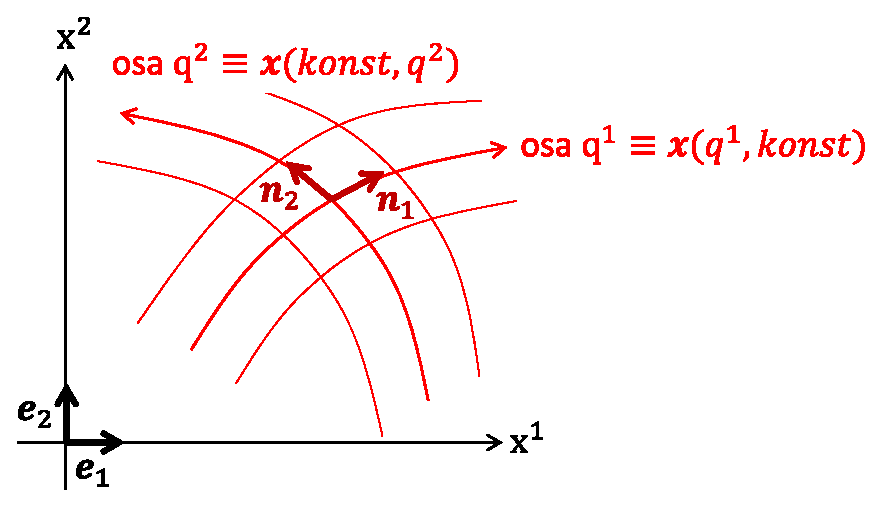
\epsfig{file=figures/coordinates.eps,width=0.66\linewidth}
    \caption{
        Ilustrace souřadnicového systému a lokální báze v křivočarých souřadnicích 
        $(q^{1},q^{2})$.
    }
    \label{fig:CurvilinearCordinates}
\end{figure}

Za předpokladu, že transformace~\eqref{eq:qx} je invertibilní, tj. že existuje inverzní transformace
\begin{equation}
    \label{eq:xq}
    x^{i}=x^{i}(\vector{q}),
\end{equation}
lze v bodě $\vector{x}$ zavést novou bázi ve směru tečen k jednotlivým souřadnicovým čarám $\axis{q}^{i}$, viz obrázek~\ref{fig:CurvilinearCordinates}\footnote{
    Souřadnicová čára $\axis{q}^{i}$ procházející bodem $\vector{Q}=(Q^{1},Q^{2},\dotsc,Q^{d})$ je definována jako čára $\axis{q}^{i}\equiv\vector{x}(q^{1}=Q^{1},\dotsc,q^{i},\dotsc,q^{d}=Q^{d})$ (tento zápis vyjadřuje, že se mění pouze souřadnice $q^{i}$, ostatní souřadnice zůstávají konstantní).
}:
\begin{equation}
    \label{eq:Vectorn}
    \vector{n}_{(i)}=\partialderivative{\vector{x}}{q^{i}}=\partialderivative{x^{j}}{q^{i}}\vector{e}_{(j)}\,;
\end{equation}
jednotlivé složky bázových vektorů $\vector{n}_{(i)}$ tedy jsou
\begin{equation}
    n_{(i)}^{j}=\partialderivative{x^{j}}{q^{i}}\,.
\end{equation}
Je třeba mít na paměti, že zatímco bázové vektory $\vector{e}_{(i)}$ jsou konstantní, bázové vektory $\vector{n}_{(i)}$ obecně závisejí na místě v prostoru: 
$\vector{n}_{(i)}=\vector{n}_{(i)}(\vector{q})$.

	\sec{Jakobián}
	Přechod mezi jednotlivými souřadnými systémy $\vector{x}$ a $\vector{q}$ je dán~\emph{Jacobiho maticí}\index{matice!Jacobiho}
	\begin{equation}
		\matrix{J}=\left(\partialderivative{\vector{x}}{\vector{q}}\right)
			=\left(\partialderivative{\left(x^{1},x^{2},\dotsc,x^{d}\right)}
            {\left(q^{1},q^{2},\dotsc,q^{d}\right)}\right)
            =\makematrix{
                \partialderivative{x^{1}}{q^{1}} & \partialderivative{x^{1}}{q^{2}} & \partialderivative{x^{1}}{q^{3}} & \\
                \partialderivative{x^{2}}{q^{1}} & \partialderivative{x^{2}}{q^{2}} & \partialderivative{x^{2}}{q^{3}} & \ldots \\
                \partialderivative{x^{3}}{q^{1}} & \partialderivative{x^{3}}{q^{2}} & \partialderivative{x^{3}}{q^{3}} & \\
                & \vdots & & \ddots
            }
	\end{equation}
	či ve složkách
	\begin{equation}
		\label{eq:JacobiMatrix}
		J_{i}^{j}=\partialderivative{x^{j}}{q^{i}}\equiv n_{(i)}^{j}\,.
	\end{equation}
	(Jacobiho matice má tedy ve sloupcích kovariantní bázové vektory $\vector{n}_{(i)}$.)
	Podmínka invertovatelnosti~\eqref{eq:xq} souvisí s nesingularitou Jacobiho matice,
	\begin{equation}
		\det{\matrix{J}}\neq 0
	\end{equation}
	($\det{\matrix{J}}$ se nazývá \emph{Jakobián}\index{Jakobián}).
	
	\sec{Duální báze}
	K bázi $\vector{e}_{i}$ se zavádí duální \emph{(kontravariantní)} báze\index{báze!kontravariantní} $\vector{e}^{(j)}$ vztahy ortogonality
	\begin{equation}
		\vector{e}_{(i)}\cdot\vector{e}^{(j)}=\delta_{i}^{j},
	\end{equation}
	kde symbol $\cdot$ udává skalární součin:\index{součin!skalární}
	\begin{equation}
		\vector{a}\cdot\vector{b}=a^{i}b_{i}\left(=\sum_{i=1}^{d}a^{i}b_{i}\right).
	\end{equation}
	Pro křivočaré souřadnice je duální báze dána vektory kolmými k plochám $q^{i}=\const$, tj. je určena gradientem
	\begin{equation}
		\vector{n}^{(i)}=\nabla q^{i}=\partialderivative{q^{i}}{x^{j}}\vector{e}^{(j)}.
	\end{equation}
    Vektory kovariantní a kontravariantní báze jsou na sebe kolmé,
	\begin{equation}
		\label{eq:DualBasisOrthogonality}
		\important{\vector{n}_{(i)}\cdot\vector{n}^{(j)}=\delta_{i}^{j}},
	\end{equation}
    což vyplývá ze zavedení obou bází:
	\begin{equation}
		\vector{n}_{(i)}\cdot\vector{n}^{(j)}
			=\partialderivative{x^{k}}{q^{i}}\vector{e}_{(k)}\cdot\partialderivative{q^{j}}{x^{l}}\vector{e}^{(l)}
			=\partialderivative{x^{k}}{q^{i}}\partialderivative{q^{j}}{x^{l}}\delta_{l}^{k}=\partialderivative{q^{j}}{q^{i}}=\delta_{i}^{j}.
	\end{equation}

	\sec{Metrický tenzor}
	Metrický tenzor\index{tenzor!metrický} se nazývá matice $\matrix{g}$ s elementy
	\begin{equation}
		\label{eq:MetricTensor}
		\boxed{g_{ij}=\vector{n}_{(i)}\cdot\vector{n}_{(j)}
			=\sum_{k=1}^{n}\partialderivative{x^{k}}{q^{i}}\partialderivative{x^{k}}{q^{j}}}.
	\end{equation}
	Z definice vyplývá, že matice $\matrix{g}$ je symetrická:
	\begin{equation}
		g_{ij}=g_{ji}.
	\end{equation}
	
	Pomocí metrického tenzoru lze spouštět indexy u kontravariantních komponent.
    Působení $\matrix{g}$ na složky libovolného vektoru $\vector{a}=a^{j}\vector{n}_{(j)}=a_{i}\vector{n}^{(i)}$ dá	
	\begin{equation}
		g_{ij}a^{j}
			=\vector{n}_{(i)}\cdot\vector{n}_{(j)}a^{j}
			=\vector{n}_{(i)}\cdot\vector{n}^{(j)}a_{j}
			=\delta_{i}^{j}a_{j}=a_{i}
	\end{equation}
	(ve třetí rovnosti jsme využili vztahu~\eqref{eq:DualBasisOrthogonality}).
	
    K matici $\matrix{g}$ se zavádí inverzní matice $\matrix{g}^{-1}$ se složkami $g^{jk}$,
	\begin{equation}
		g_{ij}g^{jk}=\delta_{i}^{k}.
	\end{equation}
	Tento inverzní metrický tenzor slouží ke zvedání indexů kovariantních komponent.

	Metrický tenzor~\eqref{eq:MetricTensor} lze získat z Jacobiho matice~\eqref{eq:JacobiMatrix} 
	\begin{equation}
        \label{eq:MetricTensorJacobi}
		\boxed{\matrix{g}=\matrix{J}^{\ti{T}}\matrix{J}}.
	\end{equation}


	\sec{Gradient}
	Gradient skalárního pole v křivočarých souřadnicích $f=f(\vector{q})$ je vektor
	\begin{equation}
		\label{eq:Gradient}
		\gradient f=\nabla f=\partialderivative{f}{q^{i}}\vector{n}^{(i)}.
	\end{equation}

	\sec{Kovariantní derivace}
Je zadáno vektorové pole v křivočarých souřadnicích $\vector{F}=\vector{F}(\vector{q})=F^{k}(\vector{q})\vector{n}_{(k)}$.
Derivování podle $i$-té složky vede na
\begin{equation}
	\label{eq:CovariantVector}
	\partialderivative{\vector{F}}{q^{i}}
		=\partialderivative{}{q^{i}}\left(F^{k}\vector{n}_{(k)}\right)
		=\partialderivative{F^{k}}{q^{i}}\vector{n}_{(k)}
			+\underbrace{\partialderivative{\vector{n}_{(k)}}{q^{i}}F^{k}}_{\partialderivative{\vector{n}_{(j)}}{q^{i}}F^{j}}
		=\partialderivative{F^{k}}{q^{i}}\vector{n}_{(k)}+\Gamma_{ij}^{k}F^{j}\vector{n}_{(k)},
\end{equation}
kde poslední rovnost plyne z toho, že $\partial\vector{n}_{(j)}/\partial q^{i}$ je vektor, a dá se tudíž vyjádřit v bázi $\vector{n}_{(k)}$ pomocí koeficientů $\Gamma_{ij}^{k}$,
\begin{equation}
	\label{eq:ChristoffelSymboln}
	\partialderivative{\vector{n}_{(j)}}{q^{i}}=\Gamma_{ij}^{k}\vector{n}_{(k)}.
\end{equation}	
Koeficienty $\Gamma_{ij}^{k}$ se nazývají \emph{Christoffelovy symboly}\index{symboly!Christoffelovy} (2. druhu).
Jsou symetrické vůči záměně dolních indexů\footnote{
	Je vidět z~\eqref{eq:Vectorn} a~\eqref{eq:ChristoffelSymboln}:
	\begin{equation}
		\partialderivative{\vector{n}_{(j)}}{q^{i}}
			=\frac{\partial^{2}\vector{x}}{\partial q_{j}\partial q^{i}}
			=\partialderivative{\vector{n}_{(i)}}{q^{j}}.
	\end{equation}
}
\begin{equation}
	\Gamma_{ij}^{k}=\Gamma_{ji}^{k}
\end{equation}
a dají se vyjádřit pomocí derivací metrického tenzoru\footnote{
	Odvození spočívá v derivování~\eqref{eq:MetricTensor} s různě označenými indexy.
}
\begin{equation}
	\label{eq:ChristoffelSymbol}
	\boxed{\Gamma_{ij}^{k}
	=\frac{1}{2}g^{kl}\left(\partialderivative{g_{il}}{q^{j}}+\partialderivative{g_{jl}}{q^{i}}-\partialderivative{g_{ij}}{q^{l}}\right)}.
\end{equation}

Rovnice~\eqref{eq:CovariantVector} zapsaná ve složkách zní
\begin{equation}
	\label{eq:CovariantDerivative}
	\boxed{{F^{k}}_{;i}=\partialderivative{F^{k}}{q^{i}}+\Gamma_{ij}^{k}F^{j}}
\end{equation}
a nazývá se \emph{kovariantní derivace}\footnote{
	Kovariantní derivace podle $i$-té složky se značí středníkem následovaným indexem $i$.
	Obyčejná derivace se značí čárkou následovanou indexem $i$.
	Rovnici~\eqref{eq:CovariantDerivative} lze tedy zapsat jako
	\begin{equation}
		{F^{k}}_{;i}={F^{k}}_{,i}+\Gamma^{k}_{ij}F^{j}.
	\end{equation}
}.

	\sec{Divergence}
Divergenci v křivočarých souřadnicích odvodíme z kovariantní derivace:
\begin{equation}
	\divergence{\vector{F}}
		={F^{k}}_{;k}
		=\partialderivative{F^{k}}{q^{k}}+\Gamma^{k}_{kj}F^{j}.
\end{equation}
Zúžený Christoffelův symbol je
\begin{equation}
	\Gamma^{k}_{kj}
		=\frac{1}{2}g^{kl}\left(\partialderivative{g_{kl}}{q^{j}}
			+\underbrace{\partialderivative{g_{jl}}{q^{k}}-\partialderivative{g_{kj}}{q^{l}}}_{0}\right)
		=\frac{1}{2}g^{kl}\partialderivative{g_{kl}}{q^{j}}
		=\frac{1}{2}\trace{\matrix{g}^{-1}\partialderivative{\matrix{g}}{q^{j}}}
\end{equation}
(druhý a třetí člen závorky jsou antisymetrické vůči záměně $k\leftrightarrow l$, 
takže při násobení symetrickou maticí $g^{kl}$ dají nulu)
a použití vztahu~\eqref{eq:LogDet} dá
\begin{equation}
	\Gamma^{k}_{kj}
		=\frac{1}{2}\partialderivative{}{q^{j}}\ln{\det{\matrix{g}}}
		=\frac{1}{2\det{\matrix{g}}}\partialderivative{}{q^{j}}\det{\matrix{g}}
		\left(=\partialderivative{}{q^{j}}\ln{\sqrt{\det{\matrix{g}}}}\right),
\end{equation}
takže
\begin{equation}
	\label{eq:Divergence}
	\divergence{\vector{F}}
		=\partialderivative{F^{k}}{q^{k}}+\left(\frac{1}{2\det{\matrix{g}}}\partialderivative{}{q^{j}}\det{\matrix{g}}\right)F^{j}
		=\frac{1}{\sqrt{\det{\matrix{g}}}}\partialderivative{}{q^{k}}\sqrt{\det{\matrix{g}}}\,F^{k}\,,
\end{equation}
přičemž poslední rovnost se dokáže rozderivováním součinu 
(jak $\det{\matrix{g}}$, tak $F^{k}$ závisejí na $\vector{q}$).

	\sec{Laplace}
Laplaceův operátor $\Delta\equiv\divergence\,\gradient$ 
získáme zkombinováním~\eqref{eq:Gradient} a~\eqref{eq:Divergence}:
\begin{equation}
	\Delta f=\frac{1}{\sqrt{\det{\matrix{g}}}}\partialderivative{}{q^{k}}\sqrt{\det{\matrix{g}}}\,g^{kl}\partialderivative{f}{q^{l}},
\end{equation}
takže samotný diferenciální operátor je
\begin{equation}
	\label{eq:Laplace}
	\boxed{\Delta
		=\frac{1}{\sqrt{\det{\matrix{g}}}}\partialderivative{}{q^{k}}\sqrt{\det{\matrix{g}}}\,g^{kl}\partialderivative{}{q^{l}}}.
\end{equation}


	\sec{Lagranžián a Hamiltonián}
Lagranžián se v obecných křivočarých souřadnicích zapisuje jako
\begin{equation}
	\label{eq:LagrangianCurvilinear}
		L(\dot{\vector{q}},\vector{q})=T(\dot{\vector{q}},\vector{q})-V(\vector{q})
			=\frac{1}{2}Mg_{kl}(\vector{q})\dot{q}^{k}\dot{q}^{l}-V(\vector{q}),
\end{equation}
kde předpokládáme, že kinetický člen systému lze zapsat jako kvadratickou formu 
v rychlostech $\dot{\vector{q}}$.
K Hamiltoniánu přejdeme zavedením zobecněných hybností
\begin{equation}
	p_{k}=\partialderivative{L}{\dot{q}^{k}}=Mg_{kl}\dot{q}^{l},
\end{equation}
takže
\begin{equation}
	\label{eq:HamiltonianCurvilinear}
	H(\vector{p},\vector{q})
		=T(\vector{p},\vector{q})+V(\vector{q})
		=\frac{1}{2M}g^{kl}(\vector{q})p_{k}p_{l}+V(\vector{q}).
\end{equation}
Nuance zavedení kvantového Hamiltoniánu jsou diskutovány v práci~\cite{Podolsky1928}.

	\sec{Schrödingerova rovnice v křivočarých souřadnicích}
	Schrödingerova rovnice v operátorové formě zní
	\begin{align}
		\operator{H}\ket{\psi}&=E\ket{\psi}\\
		\left(\frac{1}{2M}\vector{\operator{p}}^{2}+\operator{V}\right)&=E\ket{\psi},
	\end{align}
	což v $x$-reprezentaci a v křivočarých souřadnicích $\vector{q}$ vede na
	\begin{equation}
		\label{eq:SchrodingerCurvilinear}
		\left(-\frac{\hbar^{2}}{2M}\Delta+V(\vector{q})\right)\psi(\vector{q})=E\psi(\vector{q}),
	\end{equation}
	kde se za Laplaceův operátor $\Delta$ dosadí~\eqref{eq:Laplace}.

\begin{note}
	Hmotnost, či obecněji \emph{tenzor zobecněné hmotnosti}\footnote{
		Zobecněné proto, že nemusí mít rozměr hmotnosti, a tenzor proto, že může být v různých směrech různá, např. v případu rotací a tenzoru setrvačnosti, viz příklad~\ref{sec:BodyRotation}.		
	}
	lze zahrnout do metrického tenzoru, potažmo formálně do definice křivočarých souřadnic.
	Vztahy~\eqref{eq:LagrangianCurvilinear}---\eqref{eq:SchrodingerCurvilinear} pak přejdou na
	\begin{align}
		L(\dot{\vector{q}},\vector{q})
			&=\frac{1}{2}g_{kl}(\vector{q})\dot{q}^{k}\dot{q}^{l}-V(\vector{q}),\nonumber\\
		p_{k}
			&=g_{kl}\dot{q}^{l},\nonumber\\
		H(\dot{\vector{q}},\vector{q})
			&=\frac{1}{2}g^{kl}(\vector{q})p_{k}p_{l}+V(\vector{q}),\nonumber\\
		\left(-\frac{\hbar^{2}}{2}\Delta+V(\vector{q})\right)\psi(\vector{q})
			&=E\psi(\vector{q}).
		\label{eq:LagrangianHamiltonianCurvilinearM}
	\end{align}
	V případě sférických souřadnic $(r,\theta,\phi)$ to znamená zavést křivočaré souřadnice jako
	\begin{align*}
		x&=r\sqrt{M}\sin\theta\cos\phi\\
		y&=r\sqrt{M}\sin\theta\sin\phi\\
		z&=r\sqrt{M}\cos\theta.
	\end{align*}
\end{note}

	\sec{Skalární součin vlnových funkcí}
Vlnová funkce v křivočarých souřadnicích $\psi(\vector{q})\equiv\braket{\vector{q}}{\psi}$
je normalizovaná ke skalárnímu součinu
\begin{equation}
	\braket{\psi_{1}}{\psi_{2}}
		=\int\psi_{1}^{*}(\vector{q})\psi_{2}(\vector{q})\abs{\det\matrix{J}}\d\vector{q}
		=\int\psi_{1}^{*}(\vector{q})\psi_{2}(\vector{q})\sqrt{\det\matrix{g}}\,\d\vector{q}.
\end{equation}


\note
	Kvantování v křivočarých souřadnicích se dále věnují práce~\cite{Simon1965,Gruber1971,Leaf1979,Leaf1980}.

\end{theory}

\subsection{Determinant a stopa}
\begin{enumerate}
\item
	Dokažte, že pro diagonalizovatelnou matici $\matrix{A}$ platí vztah
	\begin{equation}
		\label{eq:DetExp}
		\det\e^{\matrix{A}}=\e^{\trace\matrix{A}}.
	\end{equation}
	
\item
	Na základě předchozího vztahu ukažte, že pokud je matice $\matrix{B}$ funkcí 
	zobecněných souřadnic, $\matrix{B}=\matrix{B}(\vector{q})$, platí
	\begin{equation}
		\label{eq:LogDet}
		\partialderivative{}{q^{i}}\ln\det\matrix{B}(\vector{q})=\trace\matrix{B}^{-1}(\vector{q})\partialderivative{}{q^{i}}\matrix{B}(\vector{q}),
	\end{equation}
	kde $\matrix{B}^{-1}(\vector{q})$ je matice inverzní k matici $\matrix{B}(\vector{q})$.
\end{enumerate}

\begin{solution}
	\begin{enumerate}
		\item
			Matici $\matrix{A}$ lze zdiagonalizovat a vyjádřit ve tvaru
			\begin{equation}
				\matrix{A}=\matrix{C}\matrix{D}\matrix{C}^{-1},
			\end{equation}
			kde $\matrix{D}$ je diagonální matice.
			Dosazením do~\eqref{eq:DetExp} dostaneme na levé a pravé straně
			\begin{align}
				\det{\e^{\matrix{A}}}
					&=\det{\e^{\matrix{C}\matrix{D}\matrix{C}^{-1}}}
					 =\det{\matrix{C}\e^{\matrix{D}}\matrix{C}^{-1}}
					 =\det{\matrix{C}}\det\e^{\matrix{D}}\frac{1}{\det{\matrix{C}}}\nonumber\\
					&=\det{\matrix{D}}=\prod_{j}\e^{D_{jj}},\\
				\e^{\trace{\matrix{A}}}
					&=\e^{\trace{\matrix{C}\matrix{D}\matrix{C}^{-1}}}
					 =\e^{\trace{\matrix{D}}}
					 =\e^{\sum_{j}D_{jj}}
					 =\prod_{j}\e^{D_{jj}},
			\end{align}
			čímž je~\eqref{eq:DetExp} dokázáno.
		
		\item
			Označme $\matrix{B}(\vector{q})=\e^{\matrix{A}(\vector{q})}$, 
			takže $\matrix{A}(\vector{q})=\ln{\matrix{B}(\vector{q})}$.
			Dosadíme-li do~\eqref{eq:DetExp}, dostaneme
			\begin{equation}
				\det{\matrix{B}(\vector{q})}=\e^{\trace\ln{\matrix{B}(\vector{q}})},
			\end{equation}
			po zlogaritmování
			\begin{equation}
				\ln\det{\matrix{B}(\vector{q})}=\trace\ln{\matrix{B}(\vector{q})}
			\end{equation}
			a zderivování
			\begin{equation}
				\partialderivative{}{q^{i}}\ln\det{\matrix{B}(\vector{q})}=\trace{\partialderivative{}{q^{i}}\ln{B(\vector{q})}}=\trace{\frac{1}{B(\vector{q})}\partialderivative{}{q^{i}}B(\vector{q})}.
			\end{equation}
			Tím je důkaz hotov.
	\end{enumerate}
\end{solution}

\subsection{Sférické souřadnice}
	\label{sec:SphericalCoordinates}
	Pro sférické souřadnice $\left(q^{1},q^{2},q^{3}\right)\equiv(r,\theta,\phi)$ definované běžným způsobem jako
	\begin{align}
		x&=r\sin\theta\cos\phi\nonumber\\
		y&=r\sin\theta\sin\phi\\
		z&=r\cos\theta\nonumber
	\end{align}
	vypočítejte:
	\begin{enumerate}
	\item 
		Jacobiho matici $\matrix{J}\equiv\frac{\partial(x,y,z)}{\partial(r,\theta,\phi)}$.

	\item 
		Determinant Jacobiho matice $\det\matrix{J}$.

	\item 
		Metrický tenzor $\matrix{g}$.

	\item 
		Inverzní metrický tenzor $\matrix{g}^{-1}$.

	\item 
		Determinant metrického tenzoru $\det\matrix{g}$.

	\item
		Lagranžián a Hamiltonián klasického systému bez potenciálu.

	\item 
		Laplaceův operátor $\Delta$.
	\end{enumerate}
	
\begin{solution}
	\begin{enumerate}
	\item
		Jacobiho matice podle definičního vztahu~\eqref{eq:JacobiMatrix}:
		\begin{equation}
			\matrix{J}=\makematrix{
                \sin{\theta}\cos{\phi} & r\cos{\theta}\cos{\phi} & -r\sin{\theta}\sin{\phi} \\
                \sin{\theta}\sin{\phi} & r\cos{\theta}\sin{\phi} & r\sin{\theta}\cos{\phi} \\
                \cos{\theta}  & -r\sin{\theta} & 0}.
		\end{equation}
		
	\item
		Jakobián
		\begin{align}
			\det{\matrix{J}}
				&=r^{2}\sin{\theta}\cos^{2}{\theta}\cos^{2}{\phi}+r^{2}\sin^{3}\theta\sin^{2}\phi\nonumber\\
				&+r^{2}\sin{\theta}\cos^{2}{\theta}\sin^{2}{\phi}+r^{2}\sin^{3}\theta\cos^{2}\phi\nonumber\\
				&=r^{2}\sin{\theta}\cos^{2}\theta+r^{2}\sin^{3}\theta\nonumber\\
				&=r^{2}\sin{\theta}.
		\end{align}
	
	\item
		Složky metrického tenzoru na základě~\eqref{eq:MetricTensorJacobi}:
		\begin{subequations}
			\begin{align}
				g_{11}
					&=\sin^{2}\theta\cos^{2}\phi+\sin^{2}\theta\cos^{2}\phi+\cos^{2}\theta
					 =\sin^{2}\theta+\cos^{2}\theta
					 =1,\\
				g_{12}
					&=r\sin\theta\cos\theta\cos^{2}\phi+r\sin\theta\cos\theta\sin^{2}\phi
						-r\sin\theta\cos\theta
					 =0,\\
				g_{13}
					&=-r\sin^{2}\theta\sin\phi\cos\phi+r\sin^{2}\theta\sin\phi\cos\phi
					 =0,\\
				g_{21}
					&=g_{12}
					 =0,\\
				g_{22}
					&=r^{2}\cos^{2}\theta\cos^{2}\phi+r^{2}\cos^{2}\theta\sin^{2}\phi+r^{2}\sin^{2}\theta
					 =r^{2},\\
				g_{23}
					&=r^{2}\sin\theta\cos\theta\sin\phi\cos\phi-r^{2}\sin\theta\cos\theta\sin\phi\cos\phi
					 =0,\\
				g_{31}
					&=g_{13}
					 =0,\\
				g_{32}
					&=g_{23}
					 =0,\\
				g_{33}
					&=r^{2}\sin^{2}\theta\sin^{2}\phi+r^{2}\sin^{2}\theta\cos^{2}\phi
					 =r^{2}\sin^{2}\theta.
			\end{align}				
		\end{subequations}
		V maticovém zápisu
		\begin{equation}
			\matrix{g}=\makematrix{
                1 & 0 & 0 \\
				0 & r^{2} & 0 \\
				0 & 0 & r^{2}\sin^{2}\theta}.
		\end{equation}
		
	\item
		Metrický tenzor je diagonální\sfootnote{Je-li metrický tenzor diagonální, 
		znamená to, že zobecněné souřadnice jsou v každém místě prostoru ortogonální.},
		takže inverzní matice je dána prostou inverzí diagonálních elementů,
		\begin{equation}
			\matrix{g}^{-1}=\makematrix{
                1 & 0 & 0 \\
				0 & \frac{1}{r^{2}} & 0 \\
				0 & 0 & \frac{1}{r^{2}\sin^{2}\theta}}.
		\end{equation}
	
	\item
		Determinant diagonální matice = součin členů na diagonále
		\begin{equation}
			\det{\matrix{g}}=r^{4}\sin^{2}\theta\,.
		\end{equation}
	
	\item
		Lagranžián je dán vztahem~\eqref{eq:LagrangianCurvilinear}
		\begin{equation}
			L=\frac{1}{2}M\left(\dot{r}^{2}+\dot{\theta}^{2}r^{2}
				+\dot{\phi}^{2}r^{2}\sin^{2}\theta\right)
		\end{equation}
		a Hamiltonián~\eqref{eq:HamiltonianCurvilinear}
		\begin{equation}
			H=\frac{1}{2M}\left(p_{r}^{2}+\frac{1}{r^{2}}p_{\theta}^{2}
				+\frac{1}{r^{2}\sin^{2}\theta}p_{\phi}^{2}\right).
		\end{equation}
	
	\item
		Laplaceův operátor je dán vztah~\eqref{eq:Laplace}:
		\begin{align}
			\Delta
				&=\frac{1}{r^{2}\sin\theta}\left[\partialderivative{}{r}r^{2}\sin\theta\partialderivative{}{r}
					+\partialderivative{}{\theta}r^{2}\sin\theta\frac{1}{r^{2}}\partialderivative{}{\theta}
					+\partialderivative{}{\phi}r^{2}\sin\theta\frac{1}{r^{2}\sin^{2}\theta}\partialderivative{}{\phi}\right]\nonumber\\
				&=\frac{1}{r^{2}}\partialderivative{}{r}r^{2}\partialderivative{}{r}
					+\frac{1}{r^{2}\sin\theta}\partialderivative{}{\theta}\sin\theta\partialderivative{}{\theta}
					+\frac{1}{r^{2}\sin^{2}\theta}\partialderivative[2]{}{\phi}.
        \end{align}	
        
    \item 
        Srovnání posledních dvou výrazů vede na vyjádření komponent hybnosti~\cite{Essen1978},
		\begin{subequations}
			\begin{align}
				p_{r}&=-\im\hbar\frac{1}{r}\partialderivative{}{r}r,\\
				p_{\theta}&=-\im\hbar\left(\partialderivative{}{\theta}+\frac{1}{2}\cotg{\theta}\right),\\
				p_{\phi}&=-\im\hbar\partialderivative{}{\phi}.
			\end{align}
		\end{subequations}
    \end{enumerate}
\end{solution}
\subsection{Volná rotace axiálně symetrického tělesa}
\label{sec:BodyRotation}
V prostoru volně rotuje axiálně symetrické těleso s momenty setrvačnosti $I$ vůči ose symetrie a $J$ vůči všem ostatním osám kolmým na osu symetrie a procházejícím těžištěm.
Natočení tělesa popsáno třemi Eulerovými úhly $(\phi,\theta,\psi)$,\index{úhly!Eulerovy}přičemž $\phi\in\langle0;2\pi)$ se nazývá \emph{precesní úhel} (popisuje otáční osy $Z$ spojené s tělesem vůči ose $z$ pevné v prostoru), $\theta\in\langle0;\pi)$ je \emph{nutační úhel} (popisuje úhel, který mezi sebou svírají osy $Z$ a $z$) a $\psi\in\langle0;2\pi)$ je \emph{rotační úhel} (popisuje natočení tělesa vůči ose $Z$), viz obrázek~\ref{fig:EulerAngles}\footnote{
	V praxi se souřadné systémy zavádějí tak, že osa $Z$ koinciduje s nějakým směrem významým v tělese, např. s osou symetrie, zatímco osa $z$ koinciduje se směrem významným v prostoru, např. se směrem magnetického pole.
}.
Vektor úhlové rychlosti rotace vzhledem k souřadnému systému spojenému s tělesem je
\begin{equation}
	\vector{\Omega}
		=\makematrix{0 \\ 0 \\ \dot{\psi}}
			+\underbrace{\matrix{R}_{3}(\psi)}
				_{\makematrix{\cos{\psi} & \sin{\psi} & 0 \\ -\sin{\psi} & \cos{\psi} & 0 \\ 0 & 0 & 1}}
				\makematrix{\dot{\theta} \\ 0 \\ 0}
			+\matrix{R}_{3}(\psi)\underbrace{\matrix{R}_{1}(\theta)}
				_{\makematrix{1 & 0 & 0 \\ 0 & \cos{\theta} & \sin{\theta} \\ 
					0 & -\sin{\theta} & \cos{\theta}}}
				\makematrix{0 \\ 0 \\ \dot{\phi}}\,,
\end{equation}
kde $\matrix{R}_{3}(\psi)$ přenese uzlovou přímku,\index{přímka!uzlová} která udává osu otáčení pro úhel $\theta$, na osu $X$, a $\matrix{R}_{1}(\theta)$ natočí osu $z$ podél uzlové přímky do směru osy $Z$.
Rozepsáním dostaneme \emph{Eulerovy kinematické rovnice}\index{rovnice!Eulerovy kinematické}
\begin{equation}
	\makematrix{\Omega_{1}\\ \Omega_{2}\\ \Omega_{3}}
		=\makematrix{\sin\theta\sin\psi & \cos\psi & 0 \\ \sin\theta\cos\psi & -\sin\psi & 0 \\
			\cos\theta & 0 & 1}\makematrix{\dot{\phi}\\ \dot{\theta}\\ \dot{\psi}}\,.
\end{equation}

\begin{figure}[!htbp]
	\centering
	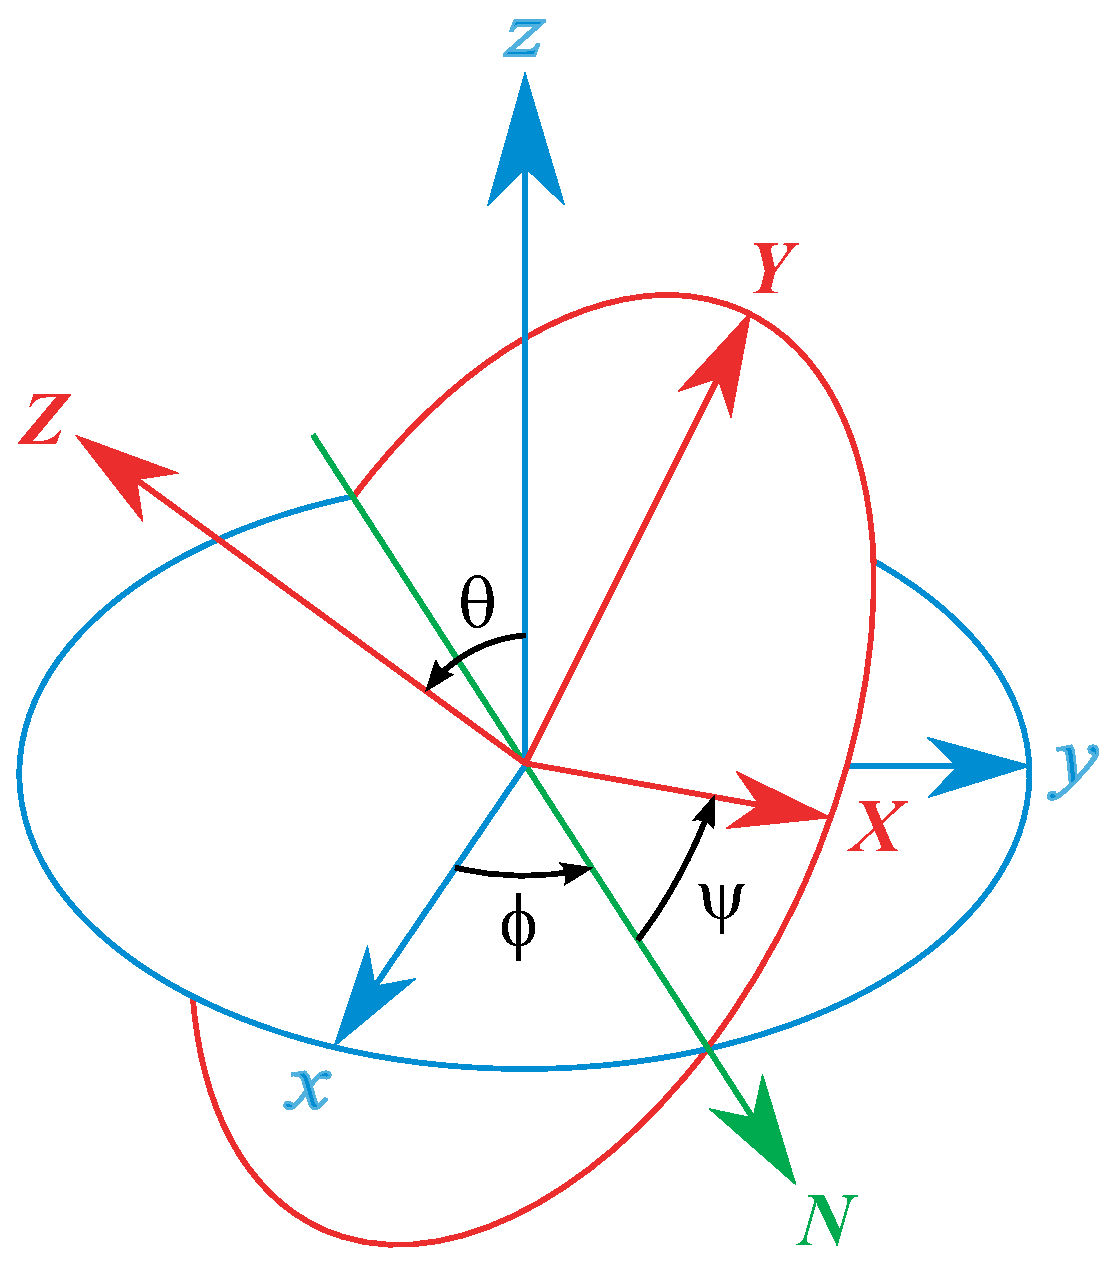
\epsfig{file=figures/euler.eps,width=0.4\linewidth}
	\caption{
		Eulerovy úhly. 
		Souřadná soustava $(x,y,z)$ pevná v prostoru (laboratorní soustava) je označena modře, souřadná soustava $(X,Y,Z)$ spojená s tělesem (těžišťová soustava) je označena červeně.
		Průsečnice rovin $(x,y)$ a $(X,Y)$, tzv. \emph{uzlová přímka}, je označena zeleně.
	}
	\label{fig:EulerAngles}
\end{figure}

\begin{enumerate}
\item 
	Napište Lagranžián za předpokladu, že osa symetrie tělesa je totožná s osou $Z$ 
	a počátek souřadné soustavy tělesa se nachází v jeho těžišti.

\item 
	Nalezněte metrický tenzor $\matrix{g}$, jeho determinant a 
	inverzní metrický tenzor $\matrix{g}^{-1}$.

\item 
	Určete Laplaceův operátor tohoto systému.

\item 
	Napište Schrödingerovu rovnici pro část závislou na úhlu $\theta$. 
	Využijte toho, že řešení Schrödingerovy rovnice lze separovat užitím substituce
	\begin{equation}
		\label{eq:BodyWaveFunction}
		u(\phi,\theta,\psi)=f(\theta)\e^{i(M\phi+K\psi)},
	\end{equation}
	kde $M$, $K$ jsou celá čísla.
\end{enumerate}
	
\begin{solution}
	\begin{enumerate}
	\item
		Pro pohyb volného tělesa je Lagranžián rovný kinetickému členu
		\begin{align}
			L&=\frac{1}{2}I\Omega_{3}^{2}
				+\frac{1}{2}J\left(\Omega_{1}^{2}+\Omega_{2}^{2}\right)\nonumber\\
			&=\frac{1}{2}I\left(\dot{\phi}\cos{\theta}+\dot{\psi}\right)^{2}
				+\frac{1}{2}J\left[\left(\dot{\phi}\sin{\theta}\sin{\psi}
				+\dot{\theta}\cos{\psi}\right)^{2}+\left(\dot{\phi}\sin{\theta}\cos{\psi}
				+\dot{\theta}\sin{\psi}\right)^{2}\right]\nonumber\\
			&=\frac{1}{2}I\left(\dot{\phi}\cos{\theta}+\dot{\psi}\right)^{2}
				+\frac{1}{2}J\left(\dot{\phi}^{2}\sin^{2}\theta+\dot{\theta}^{2}\right).
			\label{eq:BodyLagrangian}
		\end{align}
		
	\item
		V případě rotace tuhého tělesa, kdy zobecněné hmotnosti (momenty setrvačnosti) mohou být obecně v různých směrech různé, využijeme konvence~\eqref{eq:LagrangianHamiltonianCurvilinearM}.
		V našem případě je $(q^{1},q^{2},q^{3})=(\phi,\theta,\psi)$ a z~\eqref{eq:BodyLagrangian} plyne, že
		\begin{equation}
			\matrix{g}=\makematrix{I\cos^{2}\theta+J\sin^{2}\theta & 0 & I\cos{\theta} \\
						 0 & J & 0 \\
						 I\cos{\theta} & 0 & I}\,,
		\end{equation}
		\begin{equation}
			\det{g}
				=\left(I\cos^{2}\theta+J\sin^{2}\theta\right)JI-JI^{2}\cos^{2}\theta
				=IJ^{2}\sin^{2}\theta\,.
		\end{equation}
		K výpočtu inverzního metrického tenzoru využijeme vztahu
		\begin{equation}
			g^{kl}=(-1)^{k+l}\frac{\det{G_{ji}}}{\det g}\,,
		\end{equation}
		kde matici $G_{(ji)}$ získáme z matice $g$ vypuštěním $j$-tého řádku a $i$-tého sloupce.
		\begin{equation}
			\matrix{g}^{-1}
				=\makematrix{\frac{1}{J\sin^{2}\theta} & 0 & -\frac{\cos{\theta}}{J\sin^{2}\theta} \\
					0 & \frac{1}{J} & 0 \\
					-\frac{\cos{\theta}}{J\sin^{2}\theta} & 0 & 
						\frac{1}{I}+\frac{\cos^{2}\theta}{J\sin^{2}\theta}}\,.
		\end{equation}
		
	\item
		Laplaceův operátor je podle~\eqref{eq:Laplace}
		\begin{align}
			\Delta
				&=\frac{1}{J\sqrt{I}\sin{\theta}}\bigg\{\partialderivative{}{\phi}J\sqrt{I}\sin{\theta}
					\left(\frac{1}{J\sin^{2}\theta}\partialderivative{}{\phi}
					-\frac{\cos{\theta}}{J\sin^{2}\theta}\partialderivative{}{\psi}\right)\nonumber\\
				&\qquad+\partialderivative{}{\theta}J\sqrt{I}\sin{\theta}\frac{1}{J}\partialderivative{}{\theta}\nonumber\\
				&\qquad+\partialderivative{}{\psi}J\sqrt{I}\sin{\theta}
					\left[-\frac{\cos{\theta}}{J\sin^{2}\theta}\partialderivative{}{\phi}
					+\left(\frac{1}{I}+\frac{\cos^{2}\theta}{J\sin^{2}\theta}\right)
					\partialderivative{}{\psi}\right]\bigg\}\nonumber\\
				&=\frac{1}{J\sin^{2}\theta}\left[\partialderivative[2]{}{\phi}
					+\sin{\theta}\partialderivative{}{\theta}\sin{\theta}\partialderivative{}{\theta}
					-2\cos{\theta}\frac{\partial^{2}}{\partial\phi\partial\psi}
					+\left(\frac{J}{I}\sin^{2}\theta+\cos^{2}\theta\right)\partialderivative[2]{}{\psi}\right]\,.
				\label{eq:BodyLaplace}
		\end{align}
		
	\item
		Schödingerova rovnice pro vlnovou funkci~\eqref{eq:BodyWaveFunction} zní
		\begin{equation}
			-\frac{\hbar^{2}}{2}\Delta u(\phi,\theta,\psi)=Eu(\phi,\theta,\psi)\,,
		\end{equation}
		\begin{align}
			&\left[-M^{2}+\sin{\theta}\partialderivative{}{\theta}\sin{\theta}\partialderivative{}{\theta}+2MK\cos{\theta}
				-K^{2}\left(\frac{J}{I}\sin^{2}\theta+\cos^{2}\theta\right)\right]
				f(\theta)\e^{\im\left(M\phi+K\psi\right)}\nonumber\\
			&\qquad\qquad=-\frac{2J^{2}\sin^{2}\theta}{\hbar^{2}}Ef(\theta)
				\e^{\im\left(M\phi+K\psi\right)}
			\label{eq:BodySchrodinger}
		\end{align}

		Separace na část $f(\theta)$ a exponenciálu v úhlech $\phi$ a $\psi$ je možná, 
		jelikož Laplaceův operátor závisí na těchto úhlech jen přes derivace.
		Vlnová funkce musí dávat stejnou hodnotu po zvýšení $\phi$ a $\psi$ o úhel $2\pi$,
		\begin{subequations}
			\begin{align}
				u(\phi+2\pi,\theta,\psi)&=u(\phi,\theta,\psi),\\
				u(\phi,\theta,\psi+2\pi)&=u(\phi,\theta,\psi),
			\end{align}				
		\end{subequations}
		takže $M,K\in\mathbb{Z}$.
		Dá se nahlédnout, že tato vlastní čísla přísluší operátorům souvisejícím 
		s natočením okolo laboratorní osy $z$, respektive okolo osy spjaté s tělesem $Z$:
		\begin{subequations}
			\begin{align}
				\operator{M}u(\phi,\theta,\psi)&=-\im\partialderivative{}{\phi}u(\phi,\theta,\psi)=Mu(\phi,\theta,\psi)\,,\\
				\operator{K}u(\phi,\theta,\psi)&=-\im\partialderivative{}{\psi}u(\phi,\theta,\psi)=Ku(\phi,\theta,\psi)\,.
			\end{align}				
		\end{subequations}
		
		Rovnici~\eqref{eq:BodySchrodinger} převedeme na tvar
		\begin{equation}
			\label{eq:BodySchrodingerf}
			\derivative[2]{f}{\theta}+\frac{\cos{\theta}}{\sin{\theta}}\derivative{f}{\theta}
				-\frac{\left(M-K\cos{\theta}\right)^{2}}{\sin^{2}\theta}f+\sigma f=0\,,
		\end{equation}
		kde
		\begin{equation}
			\sigma=\frac{2EJ}{\hbar^{2}}-\frac{J}{I}K^{2}\,.
		\end{equation}
		V pokračování výpočtu postupujeme podle článku~\cite{Kronig1927}.
		Zavedeme substituce
		\begin{subequations}
			\begin{align}
				\lambda_{1}&=\frac{1}{2}\abs{K+M} & 
				\lambda_{2}&=\frac{1}{2}\abs{K-M} & 
				\lambda_{3}&=\frac{1}{2}+\sqrt{\frac{1}{4}+\sigma+K^{2}}\\
				\mu_{1}&=-\frac{1}{2}\abs{K+M} & 
				\mu_{2}&=-\frac{1}{2}\abs{K-M} & 
				\mu_{3}&=\frac{1}{2}-\sqrt{\frac{1}{4}+\sigma+K^{2}}
			\end{align}
			\begin{align}
				t&=\frac{1}{2}\left(\cos{\theta}+1\right)\nonumber\\
				F(t)&=\frac{f(t)}{t^{\lambda_{1}}(t-1)^{\lambda_{2}}}
			\end{align}				
		\end{subequations}
		a po dosazení do~\eqref{eq:BodySchrodingerf} dostaneme rovnici pro hypergeometrické funkce
		\begin{equation}
			t(1-t)\derivative[2]{F}{t}+\left[\gamma-(\alpha+\beta+1)t\right]\derivative{F}{t}-\alpha\beta F=0\,,
		\end{equation}
		kde
		\begin{subequations}
			\begin{align}
				\alpha&=\lambda_{1}+\lambda_{2}+\lambda_{3}\\
				\beta&=\lambda_{1}+\lambda_{2}+\mu_{3}\\
				\gamma&=2\lambda_{1}-1\,.
			\end{align}				
		\end{subequations}
		Řešení s dobrou asymptotikou dostaneme, pokud $\beta$ je nekladné celé číslo, 
		tj. $j=-\mu_{3}$ je nezáporné celé číslo.
		Dostáváme
		\begin{align}
			\left(j+\frac{1}{2}\right)^{2}&=\frac{1}{4}+\sigma+K^{2}\nonumber\\
			j(j+1)&=\sigma+K^{2}\nonumber\\
			\sigma&=j(j+1)-K^{2}\,,\nonumber
		\end{align}
		kde
		\begin{equation}
			j=(\lambda_{1}+\lambda_{2}),(\lambda_{1}+\lambda_{2}+1),\dotsc\,.
		\end{equation}
		Výsledné řešení včetně podmínek na kvantová čísla $j$, $K$, $M$ zní
		\begin{align}
			\label{eq:BodyEnergy}
			&\important{E_{jK}=\frac{\hbar^{2}}{2}\left[\frac{j(j+1)}{J}+K^{2}
				\left(\frac{1}{I}-\frac{1}{J}\right)\right]} &
			j&\in\mathbb{N}_{0}\,, & \abs{M}&\leq j\,, & \abs{K}&\leq j\,.
		\end{align}
	\end{enumerate}
				
	\begin{note}
		Spektrum volného axiálně symetrického tělesa bylo poprvé vyřešeno v práci~\cite{Kronig1927}.
	\end{note}
	
	\begin{note}
		Operátor celkového momentu hybnosti vůči soustavě spojené s tělesem 
		a jeho třetí komponenta jsou dány výrazy
		\begin{subequations}
			\begin{align}
				\operator{\mathcal{P}}^{2}
					&=-\frac{1}{\sin^{2}\theta}\left[\partialderivative[2]{}{\phi}
						+\sin{\theta}\partialderivative{}{\theta}\sin{\theta}\partialderivative{}{\theta}
						-2\cos{\theta}\frac{\partial^{2}}{\partial\phi\partial\psi}+\partialderivative[2]{}{\psi}\right]\\
				\operator{\mathcal{P}}_{3}
					&=-\im\partialderivative{}{\psi}.
			\end{align}				
		\end{subequations}
		Srovnáním s~\eqref{eq:BodyLaplace} dostaneme
		\begin{equation}
			\label{eq:tuheLaplaceP}
			\Delta=-\frac{\operator{\mathcal{P}}^{2}}{J}
				-\operator{\mathcal{P}}_{3}^{2}\left(\frac{1}{I}-\frac{1}{J}\right)
		\end{equation}
		a Schrödingerova rovnice má tvar
		\begin{equation}
			\label{eq:BodySchrodingerP}
			\frac{1}{2}\left[\frac{\operator{\mathcal{P}}^{2}}{J}
				-\operator{\mathcal{P}}_{3}^{2}\left(\frac{1}{I}-\frac{1}{J}\right)\right]
				u(\phi,\theta,\psi)=Eu(\phi,\theta,\psi)\,.
		\end{equation}
		Vlastní funkce operátoru $\operator{\mathcal{P}}^{2}$ jsou komplexně sdružené 
		Wignerovy $D$-funkce\index{funkce!Wignerovy $D$}\sfootnote{
			Wignerovy $D$-funkce ($D$-matice) jsou maticové elementy operátoru rotace
			\begin{equation}
				\operator{\mathcal{R}}(\phi,\theta,\psi)
					=\e^{-\im\psi\operator{J_{3}}}\e^{-\im\theta\operator{J_{2}}}\e^{-\im\phi\operator{J_{3}}}
			\end{equation}
			mezi vlastními stavy $\ket{jM}$ operátoru impulsmomentu a jeho třetí komponenty
			\begin{subequations}
				\begin{align}
					\operator{J}^{2}\ket{jM}&=j(j+1)\ket{jM}\\
					\operator{J}_{3}\ket{jM}&=M\ket{jM}
				\end{align}					
			\end{subequations}
			\begin{equation}
				D^{j}_{MK}(\phi,\theta,\psi)\equiv\matrixelement{jM}{\operator{\mathcal{R}}(\phi,\theta,\psi)}{jK}
					=\e^{-\im M\psi}d^{j}_{MK}(\theta)\e^{-\im K\phi}\,.
			\end{equation}
		}		
		\begin{equation}
			\operator{\mathcal{P}}^{2}D^{j*}_{MK}(\phi,\theta,\psi)
				=\hbar^{2}j(j+1)D^{j*}_{MK}(\phi,\theta,\psi)
		\end{equation}
		a působení $\operator{\mathcal{P}}_{3}$ na $D$-funkce je dáno výrazem
		\begin{equation}
			\operator{\mathcal{P}}_{3}D^{j*}_{MK}(\phi,\theta,\psi)=KD^{j*}_{MK}(\phi,\theta,\psi)\,.
		\end{equation}
		Po dosazení do~\eqref{eq:BodySchrodingerP} dostaneme spektrum~\eqref{eq:BodyEnergy} 
		a jako vlastní funkce komplexně sdružené Wignerovy $D$-funkce
		\begin{equation}
			u_{jMK}(\phi,\theta,\psi)=D^{j*}_{MK}(\phi,\theta,\psi)\,.
		\end{equation}
	\end{note}	

	\begin{note}
		Spektrum tuhého tělesa lze \uv{uhodnout} na pár řádcích.
		Hamiltonián tuhého tělesa se dá napsat jako
		\begin{align}
			\operator{H}
				&=\frac{1}{2J}\left(\operator{\mathcal{P}}_{x}^{2}+\operator{\mathcal{P}}_{y}^{2}\right)
					+\frac{1}{2I}\operator{\mathcal{P}}_{z}^{2}\nonumber\\
				&=\frac{1}{2J}\left(\vector{\operator{\mathcal{P}}}^{2}-\operator{\mathcal{P}}_{z}^{2}\right)
					+\frac{1}{2I}\operator{\mathcal{P}}_{z}^{2}\nonumber\\
				&=\frac{1}{2J}\vector{\operator{\mathcal{P}}}^{2}
					+\frac{1}{2}\left(\frac{1}{I}-\frac{1}{J}\right)\operator{\mathcal{P}}_{z}^{2},
		\end{align}
		kde $\vector{\operator{\mathcal{P}}}=\left(\operator{\mathcal{P}}_{x},\operator{\mathcal{P}}_{y},
		\operator{\mathcal{P}}_{z}\right)$ je operátor vektoru momentu hybnosti.
		Pokud předpokládáme, že jeho vlastní vektory jsou
		\begin{subequations}
			\begin{align}
				\vector{\operator{\mathcal{P}}}\ket{jK}&=\hbar^{2}j(j+1)\ket{jK}\,,\\
				\operator{\mathcal{P}}_{z}\ket{jK}&=\hbar K\ket{jK}\,,
			\end{align}				
		\end{subequations}
		dostaneme výraz~\eqref{eq:BodyEnergy}.	
	\end{note}
\end{solution}
	
\subsection{Hypersférické souřadnice}\index{souřadnice!hypersférické}
	Pro hypersférické souřadnice v prostoru o dimenzi $d$ definované vztahy
	\begin{align}
		x_{1}&=r\cos\theta_{1}\nonumber\\
		x_{2}&=r\sin\theta_{1}\cos\theta_{2}\nonumber\\
		x_{3}&=r\sin\theta_{1}\sin\theta_{2}\cos\theta_{3}\nonumber\\
		&\vdots\\
		x_{d-2}&=r\sin\theta_{1}\sin\theta_{2}\cdots\cos\theta_{d-2}\nonumber\\
		x_{d-1}&=r\sin\theta_{1}\sin\theta_{2}\cdots\sin\theta_{d-2}\cos\theta_{d-1}\nonumber\\
		x_{d}&=r\sin\theta_{1}\sin\theta_{2}\cdots\sin\theta_{d-2}\sin\theta_{d-1}\nonumber
	\end{align}
	kde $0<r<\infty$, $0\leq\theta_{j}<\pi$, $j=1,\dots,d-2$ a $0\leq\theta_{d-1}<2\pi$, vyjádřete:
	\begin{itemize}
	\item
		elementy metrického tenzoru $g_{ij}$,
	\item
		determinant metrického tenzoru $\det\matrix{g}$,
	\item 
		Laplaceův operátor~$\Delta$.
	\end{itemize}

	Ukažte, že Laplaceův operátor $\Delta$ lze rozložit na součet radiální části (závisí jen na souřadnici $r$) a části $-\frac{L_{d}^{2}}{\hbar^{2}r^{2}}$ (centrifugální člen), kde $L_{d}^{2}$ je velikost zobecněného impulsmomentu.
	Vlastí hodnoty $L_{d}^{2}$ jsou $\lambda_{d}=\hbar^{2} l_{d}(l_{d}+d-2)$, kde $l_{d}=0,1,\dots$.
	\begin{itemize}
	\item
		Vyjádřete Schrödingerovu rovnici pro radiální část vlnové funkce $R_{l_{d}}(r)$ pro sféricky symetrický potenciál $V(r)$ v $d$ dimenzích.

	\item
		Vyjádřete Schrödingerovu rovnici pro radiální část vlnové funkce $u_{l_{d}}(r)$ po substituci
		\begin{equation}
			R_{l_{d}}(r)=r^{\frac{1-d}{2}}u_{l_{d}}(r)
		\end{equation}
		a ukažte, že její tvar je shodný pro všechny dimenze $d$ a jediný rozdíl je jen ve velikosti centrifugálního členu.
	\end{itemize}

    Ukažte, že získané vztahy pro obecnou dimenzi $d$ jsou v souladu se známými vztahy pro $d=3$.

    Hypersférické souřadnice a vícerozměrný Coulombický problém jsou diskutovány v práci~\cite{Nouri1999}.
